\documentclass[12pt]{article}
\usepackage[paperwidth=25cm,paperheight=17cm,margin=1.5cm]{geometry}
\usepackage[T1]{fontenc}
\usepackage[utf8]{inputenc}
\usepackage[magyar]{babel}
\usepackage{lmodern}
\usepackage{amsmath}
\usepackage{enumitem}
\usepackage{tikz}
\usetikzlibrary{arrows.meta}

\pagestyle{empty}
\setlength{\parindent}{0pt}
\setlist[enumerate,1]{label=\textbf{\arabic*.}, leftmargin=*, itemsep=5pt, topsep=3pt}
\setlist[enumerate,2]{label=\alph*), leftmargin=2em, itemsep=1pt, topsep=1pt, parsep=0pt}

\begin{document}

\begin{center}\vspace*{-0.4cm}
  {\Large\bfseries Rezgések és mechanikai hullámok -- gyakorló feladatok}\\[4pt]
  \fbox{\parbox{0.6\textwidth}{\centering
    $g = 9{,}8~\tfrac{\text{m}}{\text{s}^2}$, \qquad
    hangsebesség levegőben: $c = 340~\tfrac{\text{m}}{\text{s}}$}}
\end{center}

\begin{enumerate}
\item \textbf{Rugós rezgő.} Egy $m = 0{,}2$~kg tömegű test $D = 80~\tfrac{\text{N}}{\text{m}}$
  rugóállandójú rugón $A = 4$~cm amplitúdóval rezeg (súrlódás nincs).
  \begin{enumerate}
    \item Mekkora a körfrekvencia, a periódusidő és a frekvencia?
    \item Mekkora a legnagyobb sebesség és a legnagyobb gyorsulás? Hol éri el ezeket a test?
    \item Mekkora a rezgés energiája? Mekkora a test sebessége $y = 2$~cm-es kitérésnél?
    \item Hogyan változik a periódusidő, a legnagyobb sebesség és az energia, ha
      \textbf{(1)} kétszer akkora tömegű testet akasztunk a rugóra (azonos amplitúdóval);
      \textbf{(2)} ugyanazt a testet kétszer akkora amplitúdóval rezegtetjük?
  \end{enumerate}
\end{enumerate}

\begin{minipage}[t]{0.58\linewidth}\vspace{0pt}
\begin{enumerate}[start=2]
\item \textbf{Grafikonelemzés.} Az ábra egy harmonikus rezgés kitérés--idő grafikonja.
  \begin{enumerate}
    \item Olvasd le az amplitúdót és a periódusidőt! Mekkora a frekvencia és a
      körfrekvencia?
    \item Mekkora a legnagyobb sebesség és a legnagyobb gyorsulás?
    \item Az első periódusban mely időpontokban nulla a sebesség? Mikor a legnagyobb a
      gyorsulás nagysága, és merre mutat ilyenkor?
    \item Rajzolj be ugyanebbe az ábrába egy ugyanilyen amplitúdójú és periódusú, de
      \textbf{ellentétes fázisú} rezgést! Mekkora annak a rezgésnek a kezdőfázisa, amelyik
      $t = 0$-kor a felső szélső helyzetben van?
  \end{enumerate}
\end{enumerate}
\end{minipage}\hfill
\begin{minipage}[t]{0.39\linewidth}\vspace{0pt}\centering
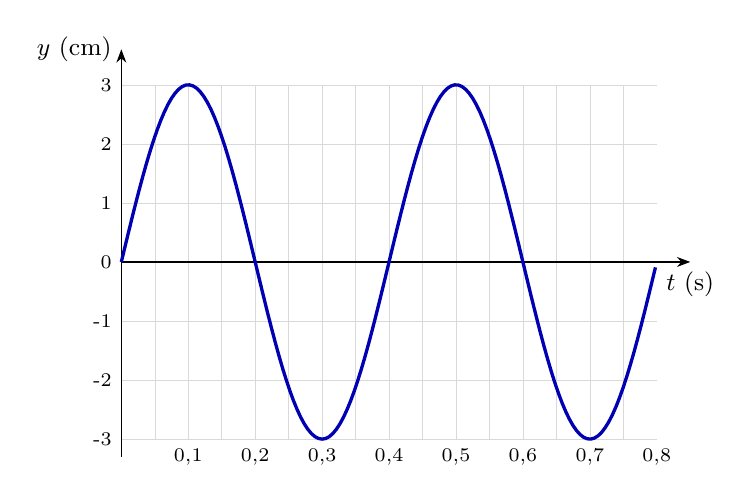
\begin{tikzpicture}[x=8.5cm,y=0.75cm,>=Stealth,font=\small]
  \draw[gray!30,very thin,xstep=0.05,ystep=1] (0,-3) grid (0.8,3);
  \draw[->] (0,0) -- (0.85,0) node[below] {$t$ (s)};
  \draw[->] (0,-3.3) -- (0,3.6) node[left] {$y$ (cm)};
  \foreach \t/\l in {0.1/0{,}1,0.2/0{,}2,0.3/0{,}3,0.4/0{,}4,0.5/0{,}5,0.6/0{,}6,0.7/0{,}7,0.8/0{,}8} \node[below,font=\scriptsize] at (\t,-3.0) {$\l$};
  \foreach \y in {-3,-2,...,3} \node[left,font=\scriptsize] at (0,\y) {\y};
  \draw[very thick,blue!70!black,domain=0:0.8,samples=150] plot (\x,{3*sin(\x/0.4*360)});
\end{tikzpicture}
\end{minipage}

\newpage
\begin{enumerate}[start=3]
\item \textbf{Fonálinga és rezonancia.}
  \begin{enumerate}
    \item Milyen hosszú az a fonálinga, amelynek periódusideje pontosan $1$~s?
    \item Mekkora lenne ugyanennek az ingának a periódusideje a Holdon
      ($g_\text{Hold} = 1{,}62~\tfrac{\text{m}}{\text{s}^2}$)?
    \item Egy $1{,}2$~m hosszú ingával $20$ teljes lengés ideje $44{,}0$~s. Mekkora ebből a
      nehézségi gyorsulás? Miért érdemes sok lengés idejét mérni egyetlen helyett?
    \item Egy hinta kötele $2{,}5$~m hosszú. Milyen időközönként kell meglökni, hogy a lengés
      egyre nagyobb legyen? Miért éppen így?
    \item A mosógép centrifugáláskor egy bizonyos fordulatszámnál erősen rázkódik, nagyobb
      fordulatszámon viszont újra nyugodtan jár. Magyarázd meg!
  \end{enumerate}
\end{enumerate}

\begin{minipage}[t]{0.58\linewidth}\vspace{0pt}
\begin{enumerate}[start=4]
\item \textbf{Hullám a kötélen.} Az ábra egy kötélen haladó hullám pillanatképe. A kötél
  végét $f = 2{,}5$~Hz frekvenciával rezgetjük.
  \begin{enumerate}
    \item Olvasd le a hullámhosszt és az amplitúdót! Mekkora a hullám terjedési sebessége és
      a kötél egy pontjának periódusideje? Mennyi idő alatt ér a hullám $10$~m-re?
    \item Transzverzális vagy longitudinális hullám az alábbiak közül melyik: kötélhullám,
      hang a levegőben, rugóban futó összenyomódás, gitárhúr rezgése? Mechanikai hullám-e a
      fény?
    \item A denevérek $40$~kHz-es ultrahanggal tájékozódnak. Mekkora ennek a hullámhossza a
      levegőben? Miért fontos, hogy ez kisebb, mint a zsákmányuk (egy rovar) mérete?
  \end{enumerate}
\end{enumerate}
\end{minipage}\hfill
\begin{minipage}[t]{0.39\linewidth}\vspace{0pt}\centering
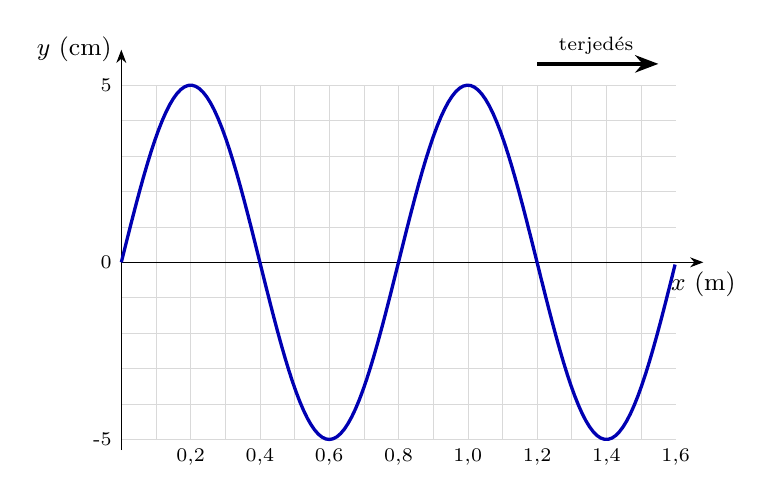
\begin{tikzpicture}[x=4.4cm,y=0.45cm,>=Stealth,font=\small]
  \draw[gray!30,very thin,xstep=0.1,ystep=1] (0,-5) grid (1.6,5);
  \draw[->] (0,0) -- (1.68,0) node[below] {$x$ (m)};
  \draw[->] (0,-5.3) -- (0,6.0) node[left] {$y$ (cm)};
  \foreach \x/\l in {0.2/0{,}2,0.4/0{,}4,0.6/0{,}6,0.8/0{,}8,1.0/1{,}0,1.2/1{,}2,1.4/1{,}4,1.6/1{,}6} \node[below,font=\scriptsize] at (\x,-5.0) {$\l$};
  \foreach \y in {-5,0,5} \node[left,font=\scriptsize] at (0,\y) {\y};
  \draw[very thick,blue!70!black,domain=0:1.6,samples=150] plot (\x,{5*sin(\x/0.8*360)});
  \draw[->,very thick] (1.2,5.6) -- (1.55,5.6);
  \node[above,font=\scriptsize] at (1.37,5.6) {terjedés};
\end{tikzpicture}
\end{minipage}

\newpage
\begin{enumerate}[start=5]
\item \textbf{Hullámtörés.} Egy $f = 2$~Hz frekvenciájú vízhullám a mély vízből
  ($c_1 = 0{,}8~\tfrac{\text{m}}{\text{s}}$) a sekély vízbe ($c_2 = 0{,}5~\tfrac{\text{m}}{\text{s}}$)
  ér, a beesési szög $40^\circ$.
  \begin{enumerate}
    \item Mekkora a hullámhossz a két részen? Melyik mennyiség nem változik, és miért?
    \item Mekkora a törési szög? A beesési merőlegeshez vagy attól törik a hullám?
  \end{enumerate}
\end{enumerate}

\begin{minipage}[t]{0.62\linewidth}\vspace{0pt}
\begin{enumerate}[start=6]
\item \textbf{Két hangszóró.} Két hangszóró azonos fázisban, $680$~Hz-es hangot ad.
  \begin{enumerate}
    \item Mekkora a hang hullámhossza?
    \item Egy hallgató az egyik hangszórótól $3{,}0$~m-re, a másiktól $4{,}25$~m-re áll.
      Hangosnak vagy halknak hallja a hangot? És ha $3{,}0$~m-re és $4{,}0$~m-re áll?
    \item Mekkora az a legkisebb útkülönbség, ahol kioltás van?
    \item Miért nem lesz egy valódi szobában a kioltási helyeken teljes csend?
  \end{enumerate}
\end{enumerate}
\end{minipage}\hfill
\begin{minipage}[t]{0.35\linewidth}\vspace{0pt}\centering
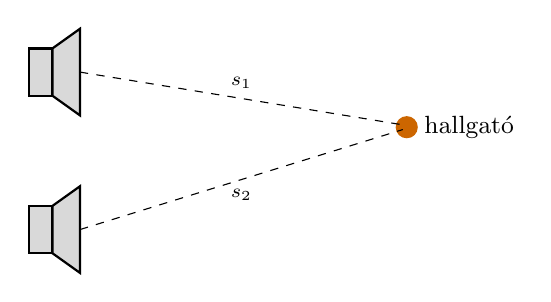
\begin{tikzpicture}[>=Stealth,font=\small]
  \foreach \y in {1,-1}{
    \draw[thick,fill=gray!30] (-0.3,\y-0.3) rectangle (0,\y+0.3);
    \draw[thick,fill=gray!30] (0,\y-0.3) -- (0.35,\y-0.55) -- (0.35,\y+0.55) -- (0,\y+0.3) -- cycle;}
  \fill[orange!80!black] (4.5,0.3) circle (4pt);
  \node[right] at (4.6,0.3) {hallgató};
  \draw[dashed] (0.35,1) -- node[above,font=\scriptsize] {$s_1$} (4.45,0.33);
  \draw[dashed] (0.35,-1) -- node[below,font=\scriptsize] {$s_2$} (4.45,0.27);
\end{tikzpicture}
\end{minipage}

\vspace{4pt}
\begin{enumerate}[start=7]
\item \textbf{Gitárhúr.} Egy $L = 0{,}6$~m hosszú gitárhúr alaphangja $330$~Hz.
  \begin{enumerate}
    \item Mekkora az alaphanghoz tartozó hullámhossz, és mekkora a hullám terjedési
      sebessége a húron?
    \item Mekkora az első két felhang frekvenciája? Rajzold le a húr alakját az első
      felhangnál, és jelöld a csomópontokat és a duzzadóhelyeket!
    \item A gitáros lefogja a húrt, így a rezgő rész $0{,}45$~m-re rövidül. Mekkora az új
      alaphang?
  \end{enumerate}

\item \textbf{Szóbeli gyakorlás.} Válassz egyet, és fejtsd ki összefüggő szövegben, 3--4
  percben: \textbf{(A)} \emph{A harmonikus rezgőmozgás} (jellemzők, kapcsolat a
  körmozgással, dinamikai feltétel, periódusidő, energia, rezonancia), vagy
  \textbf{(B)} \emph{A mechanikai hullámok} (keletkezés, fajták, jellemzők,
  visszaverődés, törés, interferencia, állóhullám, elhajlás).
\end{enumerate}

\end{document}
